\section{Monte Carlo Methods}
If we do not have knowledge of the transition probabilities (model of the environment) then we must learn directly from experience. To do so, we use Monte Carlo methods. Monte carlo methods are most effective in episodic tasks where there is a terminal state and the value of the states visited en route to the terminal state can be updated based on the reward received at the terminal state. We use general policy iteration as outlined in chapter 4, but this time instead of \textit{computing} the value function we learn it from samples. We first consider the prediction problem to obtain $v_\pi$ and/or \textbf{$q_\pi$} for a fixed policy, then we look to improve using policy improvement, then we use it for control.  

\subsection{Monte Carlo Policy Prediction}
\begin{itemize}
\item Recall that the value of a state is the expected discounted future reward from that state. One way of estimating that value is by observing the rewards obtained after visiting the state, we would expect that in the limit this would converge toward the true value.
\item We can therefore run a policy in an environment for an episode. When the episode ends, we receive a reward and we assign that reward to each of the states visited en route to the terminal state. 
\item Where DP algorithms perform one-step predictions to \textit{every} possible next state; monte-carlo methods only sample one trajectory/episode. This can be summarised in a new backup diagram as follows:
\begin{figure}[h!]
	\centering
	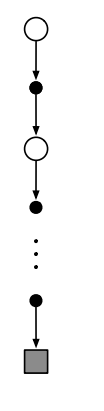
\includegraphics[width=0.1\textwidth]{/chapter5_1}
	\caption{Monte carlo backup diagram for one episode}
	\label{fig:monte carlo backup}
\end{figure}

\item Importantly, monte carlo methods do not bootstrap in the same way DP methods do. They take the reward at the end of an episode, rather than estimated reward based on the value of the next state.
\item Because of the lack of bootstrapping, this expense of estimating the value of one state is independent of the number of states, unlike DP. A significant advantage, in addition to the other advantages of being able to learn from experience without a model or from simulated experience. 
\end{itemize}

\subsection{Monte Carlo Estimation of Action Values}
\begin{itemize}
\item With a model we only need to estimate the state value function \(v\) as, paired with our model, we can evaluate the rewards and next states for each of our actions and pick the best one.
\item With model free methods we need to estimate the state-action value function \(q\) as we must explicitly estimate the value of each action in order for the values to be useful in suggesting a policy. (If we only have the values of states, and don't know how states are linked through a model, then selecting the optimal action is impossible)
\item One serious complication arises when we do not visit every state, as can be the case if our policy is deterministic. If we do not visit states then we do not observe returns from these states and cannot estimate their value. We therefore need to \textit{maintain exploration} of the state space. One way of doing so is stochastically selected a state-action pair to start an episode, giving every state-action pair a non-zero probability of being selected. In this case, we are said to be utilising \textit{\textbf{exploring starts}}.
\item Exploring starts falls down when learning from real experience because we cannot guarantee that we start in a new state-action pair in the real world. 
\item An alternative approach is to use stochastic policies that have non-zero probability of selecting each state-action pair.
\end{itemize}


\subsection{Monte Carlo Control}
\begin{itemize}
\item Much like we did with value iteration, we do not need to fully evaluate the value function for a given policy in monte carlo control. Instead we can merely \textit{move} the value toward the correct value and then switch to policy improvement thereafter. It is natural to do this episodically i.e. evaluate the policy using one episode of experience, then act greedily w.r.t the previous value function to improve the policy in the next episode.
\item If we use a deterministic policy for control, we must use exploring starts to ensure sufficient exploration. This creates the \textit{Monte Carlo ES} algorithm.
\end{itemize}

\subsection{Monte Carlo Control without Exploring Starts}
\begin{itemize}
\item To avoid having to use exploring starts we can use either \textit{on-policy} or \textit{off-policy} methods. The only way to ensure we visit everything is to visit them directly.
\item On-policy methods attempt to improve or evaluate or improve the policy that is making decisions.
\item On-policy control methods are generally \textit{soft} meaning that they assign non-zero probability to each possible action in a state e.g. e-greedy policies.
\item We take actions in the environment using e-greedy policy, after each episode we back propagate the rewards to obtain the value function for our e-greedy policy. Then we perform policy improvement by updating our policy to take the \textbf{new} greedy reward in each state. Note: based on our new value function, the new greedy action may have changed in some states. Then we perform policy evaluation using our new e-greedy policy and repeat (as per generalised policy iteration).
\item The idea of on-policy Monte Carlo control is still that of GPI. We use first visit MC methods to estimate the action-value function i.e. to do policy evaluation, but we cannot then make improve our policy merely by acting greedily w.r.t our value function because that would prevent further exploration of non-greedy actions. We must maintain exploration and so improve the $\epsilon$-greedy version of our policy. That is to say, when we find the greedy action (the action that maximises our reward for our given value function) we assign it probability $1 - \epsilon + \frac{\epsilon}{\mathcal{A}(S_t)}$ of being selected so that the policy remains stochastic.
\item Note: doing the above will only find us the best policy amongst the $\epsilon$-soft policies, which may not be the optimal policy for the environment, but it does allow us to remove the need for exploratory starts.
\end{itemize}

\subsection{Off-policy Prediction via Importance Sampling}
We face a dilemma when learning control: we want to find the optimal policy, but we can only find the optimal policy by acting suboptimally to explore sufficient actions. What we saw with on-policy learning was a compromise - it learns action values not for the optimal policy but for a near-optimal policy that still explores. An alternative is off-policy control where we have two policies: one used to generate the data (behaviour policy) and one that is learned for control (target policy). This is called \textit{off policy learning}.

\begin{itemize}
\item Off-policy learning methods are powerful and more general than on-policy methods (on-policy methods being a special case of off-policy where target and behaviour policies are the same). They can be used to learn from data generated by a conventional non-learning controller or from a human expert.
\item If we consider an example of finding target policy $\pi$ using episodes collected through a behaviour policy $b$, we require that every action in $\pi$ must also be taken, at least occasionally, by $b$ i.e. $\pi(a|s) > 0$ implies $b(a|s) > 0$. This is called the assumption of \textit{\textbf{coverage}}. 
\item Almost all off-policy methods utilize \textit{importance sampling}, a general technique for estimating expected values under one distribution given samples from another. Given a starting state $S_t$, the probability of the subsequent state-action trajectory occuring under any policy $\pi$ is:

\begin{equation}
	\prod_{k=t}^{T-1} \pi(A_k|S_k)p(S_{k+1}|S_k, A_k)
\end{equation}

where $p$ is the state transition probability function. We can then obtain the relative probability of the trajectory under the target and behaviour policies (the importance sampling ratio) as:

\begin{equation}
p_{t:T-1} = \frac{\prod_{k=t}^{T-1} \pi(A_k|S_k)p(S_{k+1}|S_k, A_k)}{\prod_{k=t}^{T-1} b(A_k|S_k)p(S_{k+1}|S_k, A_k)} = \prod_{k=t}^{T-1} \frac{\pi(A_k|S_k)}{b(A_k|S_k)}
\end{equation}

We see here that the state transition probability function helpfully cancels.

\item We want to estimate the expected returns under the target policy but we only have returns from the behaviour policy. To address this we simply multiply expected returns from the behaviour policy by the importance sampling ratio to get the value function for our target policy.

\begin{equation}
\mathbb{E} \left[p_{t:T-1} G_t | S_t = s\right] = v_\pi(s)
\end{equation}

\item Note: importance sampling ratios are only non-zero for episodes where the target-policy has non-zero probability of acting \textit{exactly} like the behaviour policy $b$. So, if the behaviour policy takes 10 steps in an episode, each of these 10 steps have to have been \textit{possible} by the target policy, else $\pi(a|s) = 0$ and $\rho_{t:T-1} = 0$.

\end{itemize}

\subsection{Incremental Implementation}
We perform monte carlo policy evaluation (prediction) incrementally in the same way as was done in Chapter 2 for the bandit problem. Generally incremental implementation follows this formula:

\begin{equation}
New Estimate \leftarrow Old Estimate + Step Size \left[Observation - Old Estimate \right]
\end{equation}

With on-policy monte carlo methods, this update is performed exactly after each episode for each visit to a state given the observed rewards, with off-policy methods the update is slightly more complex. With ordinary importance sampling, the step size is $1/n$ where $n$ is the number of visits to that state, and so acts as an average of the scaled returns. For weighted importance sampling, we have to form a weighted average of the returns which requires us to keep track of the weights. If the weight takes the form $W_i = \rho_{t:T(t)-1}$ then our update rule is:

\begin{equation} \label{incremental V}
V_{n+1} = V_n + \frac{W_n}{C_n}\left[G_n - V_n\right]
\end{equation}
where,
\begin{equation}
C_{n+1} = C_n + W_{n+1}
\end{equation}
with $C_0 = 0$. This allows us to keep tracking of the corrected weighted average term for each update as they are made. Note here that the weighted average gives more weight to updates based on common trajectories from $b$ in $\pi$ that we have some more often.

\subsection{Off-policy Monte Carlo Control}
Using incremental implementation (updates to the value function) and importance sampling we can now discuss \textit{off-policy monte carlo control}–the algorithm for obtaining optimal policy $\pi_*$ by using rewards obtained through behaviour policy $b$. This works in much the same way as in previous sections; $b$ must be $\epsilon$-soft to ensure the entire state space is explored in the limit; updates are only made to our estimate for $q_\pi$, $Q$, if the sequence of states an actions produced by $b$ could have been produced by $\pi$. This algorithm is also based on GPI: we update our estimate of $Q$ using Equation \ref*{incremental V}, then update $\pi$ by acting greedily w.r.t to our value function. If this policy improvement changes our policy such that the trajectory we are in from $b$ no longer obeys our policy, then we exit the episode and start again. The full algorithm is shown in \ref*{fig:Off-policy monte carlo control}.

\begin{figure}[h!]
	\centering
	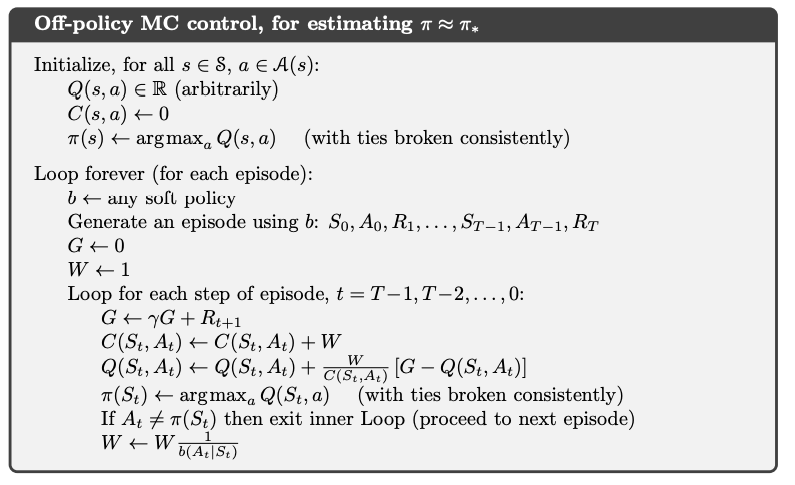
\includegraphics[width=0.5\textwidth]{/chapter5_3}
	\caption{Off-policy monte carlo control}
	\label{fig:Off-policy monte carlo control}
\end{figure}

\subsection{Key Takeaways}
\begin{itemize}
\item In the absence of a model of the environment, monte carlo methods allow us to evaluate and improve our value function based on \textit{experience}
\item We roll-out trajectories to terminal states, and back-propagate the rewards to the states visited en-route in several ways
\item Monte carlo methods use GPI (see chapter 4) in much the same way dynamic programming does. We evaluate our policy, then improve by acting greedily w.r.t our new value function until we converge on the optimal value function and policy.
\item Differences with dynamic programming methods: 1) They do not require a model of the environment as they learn directly from experience, and 2) They do not bootstrap i.e. the value function estimates are an average of all real returns accumulated after visiting the state.
\item Maintaining sufficient exploration is crucial with monte carlo methods; if our policy is deterministic we will likely not explore the full states space during our roll-outs. To deal with this we have several options: 1) Start every episode randomly with uniform probability such that we make sure we start at each possible state–called \textit{exploring starts}, unrealistic in the real world as we can't make a robot restart from all possible states. Or 2) Use $\epsilon$-soft policies that have a non-zero probability of selecting all possible states. The downside of doing this is that we will converge on the optimal $\epsilon$-soft, which is not necessarily the optimal policy for the environment, because it needs to learn how account for its own randomness. This is the price we pay for exploration.
\item Monte carlo methods can either be \textit{on-policy} or \textit{off-policy}.
\item On-policy methods use the same policy to collect data as is evaluated and improved. This suffers the downsides outlined above.
\item Off-policy methods have two policies, one that collects the data called the \textit{behaviour policy} $b$ and the other which we look to improve called the target policy $\pi$. We find trajectories from the behaviour policy that line up with our target policy, that is to say, that could have been produced by our target policy. This process only works if the behaviour policy has non-zero probability of selecting each of the actions in the target policy, aka \textit{coverage} of the target policy. The agent explores, but learns a deterministic optimal policy offline that may be unrelated to the behaviour policy used to collect the experience.
\item Based on rewards observed by running the behaviour policy, we update our value function using \textit{importance sampling}, which measures, if effect, how likely the observed behaviour would have been given our target policy. For example, the target policy may take 1 of 4 actions with equal probability in each state. If we observe two timesteps from our beaviour policy, then our probability of selecting the actions taken by the behaviour policy would be $0.25 x 0.25$. 
\item We weight each return using the x\textit{importance sampling ratio}, a measure of how likely we were to produce the roll-out using the target policy compared to how likely we were to produce the roll-out using the behaviour policy. 
\item Importance sampling can be \textit{ordinary} i.e. an average of the returns observed from a state or \textit{weighted} where trajectories viewed more often, or with a higher importance sampling ratio give the value update more weight.

\end{itemize}